
\section{Implementation}
\label{sec:impl}

\begin{table*}[t]
\centering
\begin{small}
\begin{tabular}{|l|l|l|}
\hline
\multicolumn{3}{|c|}{{\bf System Calls (batched)}} \\
\hline
connect &             cookie, dst\_IP, dst\_port		& Opens a connection\\
accept &              handle, cookie				& Accepts a connection\\
sendv &               handle, scatter\_gather\_array		& Transmits a scatter-gather array of data\\
recv\_done &          handle, bytes\_acked			& Advances the receive window and frees memory buffers\\
close &               handle					& Closes or rejects a connection\\
\hline  \hline
\multicolumn{3}{|c|}{{\bf Event Conditions}} \\
\hline
{\bf Type} &           {\bf Parameters}  &
{\bf Description}\\
knock  &               handle, src\_IP, src\_port		& A remotely initiated connection was opened \\
connected &            cookie, outcome				& A locally initiated connection finished opening \\
recv &                 cookie, mbuf\_ptr, mbuf\_len		& A message buffer was received \\
sent &                 cookie, bytes\_sent, window\_size	& A send completed and/or the window size changed \\
dead &                 cookie, reason				& A connection was terminated \\
\hline
\end{tabular}
\caption{\ix system calls and event conditions API. 
}
\label{tbl:api}
\end{small}
\end{table*}


\begin{figure}
\hspace*{-0.25in}\centering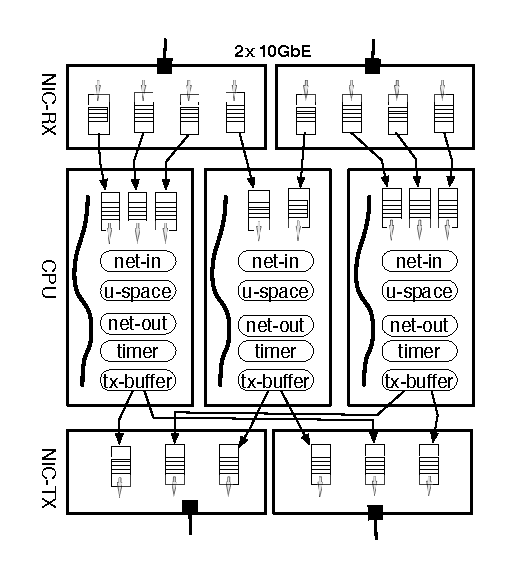
\includegraphics{figs/queues-cores.eps}
\caption{Example of IX scaling across two NICs interfaces, 8 NIC RX queues, and 3 CPU hardware threads.} 
\label{fig:queues-cores}
\end{figure}





We now describe the implementation of the \ix prototype.  We start
with an overview of the \ix kernel (\S\ref{sec:impl:kernel}), describe
the environment surrounding \ix (\S\ref{sec:impl:env}), and explain
what makes \ix more efficient (\S\ref{sec:impl:better}).
We close with a
discussion of our approach, its current implementation restrictions,
and directions for future work (\S\ref{sec:impl:discussion}).


%the benefits of having \ix run as a guest
%operating system (\S\ref{sec:impl:guest}), its native API at the
%kernel/user boundary (\S\ref{sec:impl:api}), the implementation of the
%networking stack (\S\ref{sec:impl:stack}), the implications on
%congestion management and flow control (\S\ref{sec:impl:net}), the
%benefits and consequences of coherence-free execution
%(\S\ref{sec:impl:cohfree}), and finally our approach to compatibility
%(\S\ref{sec:impl:libix}).


\subsection{The \ix Kernel}
\label{sec:impl:kernel}



The \ix kernel consists of 37 KSLOC (according to SLOCcount
2.26~\cite{url:sloccount}), of which 43\% is derived from the Intel
device driver, 23\% from the lwIP TCP stack, and 16\% from the Dune
library and sandboxing module.  All three existing code bases are
highly modified for the purpose; the rest is approximately 7KSLOC of
new code.  The \ix kernel merges two distinct functions, as it is both
an operating system and a dataplane.

\myparagraph{Control flow:} \ix is an single address-space OS that can launch and run a single
legacy, multi-threaded POSIX application. \ix supports two distinct
thread types within the shared, userlevel address space: (i)
\emph{elastic threads} which interact with the \ix kernel to initiate
and consume network I/O and (ii) \emph{background threads} who can
issue arbitrary POSIX calls, including ones with blocking conditions.
Elastic threads interact essentially interact with the kernel through
three asynchronous, non-blocking mechanisms: they consume \emph{event
  conditions} generated by the kernel, have a direct, but safe, access
to message buffers \emph{mbuf}) containing incoming networking
payload, and can issue \emph{batched systems calls} to the kernel.

\myparagraph{Run to completion:} 
Fig.~\ref{fig:queues-cores} illustrates the run-to-completion model of the
dataplane for a multi-NIC, multi-queue and multi-core configuration.
Hardware NIC queues are assigned to elastic threads, which run
independently.  The elastic thread (i) polls the receive queues of the
NIC to dequeue all newly received packets into an in-memory queue, and
post fresh descriptors; 
 (ii) processes a bounded number of packets
through the incoming networking stack, thereby generating event
conditions; (iii) passes control to the user-space applications, which
consumes all event conditions, and in return responds with a batch of
system calls; (iv) upon return of control from user-space, \ix
processes all system calls, and in particular the ones that direct
outgoing networking traffic; (v) run all kernel timers, in particular
to ensure compliant TCP behavior; (vi) ensures that all outgoing
Ethernet frames can be put into NIC TX descriptor rings.

\myparagraph{API:} 
Table~\ref{tbl:api} enumerates the most important event conditions and
batched system calls of \ix.  Unlike a traditional OS with POSIX
sockets, \ix directly (but safely) exposes message buffers to
applications for a zero-copy access to the incoming payload.
Applications can then hold on to message buffers and release them via
a batched system call.  \ix also differs in directly exposing flow
control conditions to application: the \texttt{sendv} batched system
call does not synchronously return the number of bytes sent; instead,
the \texttt{Recv} event condition provides that infromation in a
subsequent step.

\adam{I think we should talk a little more about the mechansims behind batching
and event conditions because they are unusual compared to previous systems.}


\subsection{The environment}
\label{sec:impl:env}

\begin{figure}
\begin{centering}
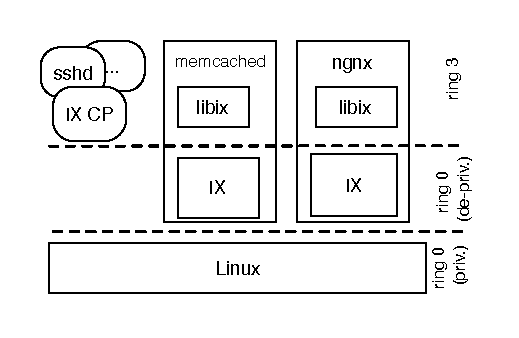
\includegraphics{figs/cp-dp.eps}
\centering\caption{Protection and separation in \ix.}
\label{fig:cp-dp}
\end{centering}
\end{figure}



Fig.~\ref{fig:cp-dp} illustrates the environment that surrounds the
\ix kernel.  We rely on VT-x hardware
virtualization~\cite{DBLP:journals/computer/UhligNRSMABKLS05} to run
\ix as a guest operating system using Dune~\cite{belay2012dune}. Dune
itself runs as part of a Linux host and allows untrusted host
processes (in our case \ix) to securely access de-privileged hardware
functions.

\myparagraph{Separation and protection of control and data plane:}
Each \ix instance and its applications runs as a distinct Dune process
while control plane functions, including the control and monitoring of
dataplane, is performed by scripts and daemons of the host
environments.  This provides protection between control and
dataplanes. Within each dataplane, \ix further protects itself from
the untrusted application through virtual memory andby running it at
userlevel.

\myparagraph{Application compatibility:} We extended the Dune
sandboxing mechanisms to support the initial load of multi-threaded
applications into the userlevel address space, to launch both elastic
and background threads.  Although elastic threads could directly use
the native API of Table~\ref{tbl:api}, this would require a
substantial effort; the userlevel library therefore also includes a
compatibility mechanism that exposes the near-identical API as
\texttt{libevent} as the expense of \edb{TODO TODO TODO}.  Both
elastic and background threads can also issue arbitrary POSIX system
calls; those are merely intermediated by \ix, and handled by the
underlying OS.  Elastic threads are expected to \emph{not} issue blocking
system because of the adverse impact on network behavior and
performance.

\myparagraph{Resource management:}
We rely on Linux's abilty to allocate resources at a coarse grain to
demanding applications, in our case the Dune processes.  For example,
core allocation can be precisely controlled through real-time
priorities and \texttt{cpumasks}; memory can be allocated in 2MB and
1GB chunks from specified NUMA nodes; PCI devices, virtual functions,
and NIC hardware queues alike can be assigned to specified \ix
kernels, etc.  This explicitly favors scalability and performance by
muliplexing resources in space among the various dataplanes, but not
in time at a fine granularity.  For example, elastic threads are
guaranteed exclusive access to the underyling hyperthread until that
allocation is explicitly revoked, using a protocol similar to the one
used in Exokernels~\cite{DBLP:conf/sosp/EnglerKO95}.  

\myparagraph{Elasticity policies:}
In contrast to the mechanisms, which are generic, different policies
can be envisioned to meet different use cases and optimization
functions.  If neither energy proportionality or server consolidation
is of any concern, the control plane can obviously launch a single
dataplane instance configured with the maximal available physical
resources.  In more realistic scenarios, the dataplane is
``right-sized'' to meet its service-level agreements with minimal
resource allocations.  The control plane can further dynamically add
or revoke CPUs from a dataplane instances, e.g., when the dataplane
signals some sustained congestion or violation of its service-level
agreements, or conversely when the allocated CPU resources are
underutilized.

%\begin{figure}
\begin{centering}
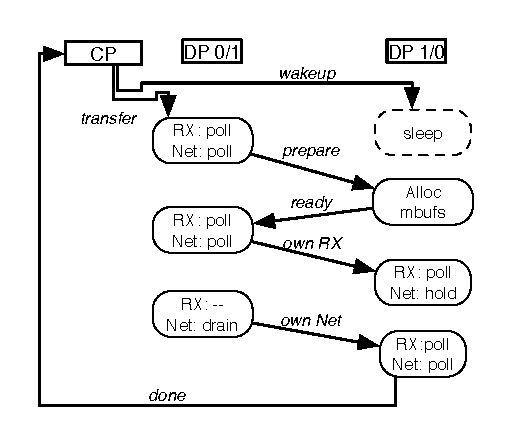
\includegraphics{figs/queue-takeover.eps}
\caption{Queue takeover algorithm.}
\label{fig:queue-takeover}
\end{centering}
\end{figure}



\subsection{What Makes \ix More Efficient?}
\label{sec:impl:better}

\adam{To me this doesn't seem like implementation... perhaps we can move this section to discussion. I like talking about this
from a lesson's learned perspective and it follows naturally to discuss perfomrance after the evalation.}

Some critical design and implementation decisions have a significant
impact on performance.

\myparagraph{Coherency-free Execution:}
According to the commutatity rule, system call implementations can
only be coherence-free if the the API itself is
commutative~\cite{DBLP:conf/sosp/ClementsKZMK13}.  Our API is
commutative: events are processed independently on each elastic thread
and flows are identified by cookies rather than a single file
descriptor snamespace.  Our implementation is free of any
cache-coherency traffic in the common case: each elastic thread
manages its own memory pools and \ix relies on flow-consistent hashing
by the NIC hardeware to ensure that each elastic thread operates on a
disjoint subset of the TCP flows. \adam{these aren't exceptions in my view.
coherence traffic on the cold path is necessary and expected.}  There are only a few exceptions to
that rule: for example, the ARP table is shared by all corees and
protected by RCU locks~\cite{mckenney1998read}, which means that
updates are not coherency-free.
\adam{lesson learned: coherence free is great for scalability but there
are other architectural bottlenecks to consider too like device access
over PCI. For example, by batching TX ring tail updates, we greatly
improved scalability. Also, lock-free data structures are not
good enough.}

\myparagraph{Redundant outbound connections:} Coherency-free execution is only possible when flows are consistently
handled by the same elastic thread for both input and output.  For
accepted connection, the RSS hardware ensures isolation and
application cannot legally share a flow descriptor cookie across core.
For outbound connections, the issue is trickier: \ix selects the
source emphemeral port based on the requesting elastic thread. Since
the Toeplitz hash function cannot be reversed, \ix simply probes the
ephemeral namespace and computes the Toepliz hash until a match is
found.  We note two side-effects: first, connections between and \ix
client and a server will be replicated for each elastic thread; second
the ephemeral ports no longer form a namespace, and an \ix client can
easily open millions of connections (to distinct servers).
\adam{Lesson learned: RSS is a bad design for affinity of outgoing
connections. An alternative might be to use flow director as described
in affinity accept.}

\myparagraph{Coupling of networking stack and application:}
A traditional in-kernel stack decouples protocol processing, which
occurs at interrupt level, from the applications which are scheduled
by the OS.  \ix keeps maintains a strongly coupling: elastic threads
intermixing protocol procesing with the non-blocking execution of the
application, and interrupts are only used as watchdogs to detect
non-cooperating applications.  This has a number of performance
benefits, notably replacing context switching with low-overhad system
call transitions.  It also removes unncessary abstractions, such as
the buffering in the socket layer.
\adam{Lesson learned: coupling causes application code to get scheduled in a way
that makes it more efficient. Just considering kernel versus user time of
existing systems shows an incomplete picture.}

\myparagraph{Zero-copy:} \ix exposes incoming message buffers directly
to applcations in a read-only portion of the address
space. Application can hold on to them until they acknowledge completion (\texttt{recv\_done}).
Similarly, \ix never copies outgoing payloads into its memory, but
instead expects the application to keep the content unmodified until
acknowledgements have been confirmed.  This obviously eliminate a
major source of data movement overhead for streaming applications.
But the approach also helps workloads with small packets as it
eliminates many memory management corner cases.
\adam{Lesson learned: A zero-copy architecture helps even
when high-level API's are not zero-copy. The key factor is cache efficiency.
By allowing the compatibility library to perform
copies instead of the kernel we get improved temporal locality, as buffers are accessed
immediately after they are copied.}

\myparagraph{Bounded, adaptive batching:} During the first stage of
its pipeline, \ix moves all incoming packets from the hardware ring
into a corresponding in-memory queue, but only process a bounded batch
of packets in all subsequent steps.  This design has a number of
benefits: (i) it ensures that \ix can sustain instaneous congestion by
making use of the extensive DRAM resource available; (ii) the
resulting in-memory queue can serve as the basis for extensive
monitoring of service-level agreement expressed in terms of queuing
delays, and provides a convenient location to implement congestion
management policies such as ECN~\cite{ramakrishnan2001addition} or
RED~\cite{DBLP:journals/ton/FloydJ93}; (iii) it offers simulatenously
low-latency reponse times when the queues are shallow and high
throughput when the queues are deeper.  In our system, we determined
experimentally that a bound as low as \george{XXX} sufficiently
amortizes overheads, even in network-intensive, CPU-bound situations.

\myparagraph{Flow control:} Bounded batching has an additional benefit
in terms of flow control, as acknowledgments are sent by the
networking stack only when packets are processed by the dataplane.
Congestion in the NIC edge therefore leads to shrinking windows in
peers.  In contrast, traditional stacks acknowledge packets well
before they are processed by application and buffer in the socket
layer.  When sending, flow control is safely, but directly exposed to
user-space applications, providing a direct view of the sliding
window, which they can use to improve their own QoS, e.g., when mixing
elephant and mice flows in a key-value store.
\adam{Lesson learned: There's no reason to provide flow control
in the kernel as applications can make better decisions directly.}


\subsection{Discussion}
\label{sec:impl:discussion}

We now move to a discussion of certain open issues, tradeoffs,
implementation limitations of our prototype, and discussion of future
work.

\myparagraph{The \ix TCP stack:} 
The \ix kernel includes a complete network protocol stack with
RFC-compliant support for TCP, UDP, ARP, ICMP and LACP.  It however
explicitly lacks a complete IP-layer and is therefore only a capable
networking endpoint, but not of handling routing, bridging or
filtering functions.  It also totally lacks a socket layer and its
associated API and semantics.  For our implementation of TCP, we chose
to lwIP~\cite{dunkels2001design} as a starting point for our code base because of its
modularity and is maturity as a compliant, feature-rich networking
stack.  lwIP was however designed with memory-efficiency in mind,
primarily for embedded environments.  We radically changed the data
structures that organize protocol control blocks for scalability, as
well as for finer-grain, precise timer management.  However, we did
not (yet) attempt to optimize the code paths for performance, and
consequently believe that our results have room for improvement.

\myparagraph{Limitations of the prototype:} 
The \ix prototype is architected to support any stateless offload NIC
with multiple queues and support for flow-consistent hashing in
hardware (e.g., RSS).  However, we've only ported the Intel XXX
driver, using DPDK~\cite{intel:dpdk} as a starting code base.  We
avoided adding to \ix a Linux driver compatibilty, explicitly trading
off higer portability costs for higher performance.  Because of
restrictions in the use of VT-d in particular in the area of
\adam{XXXX}, the device operates without an IOMMU.  Instead, the
driver directly populates descriptors with host-physical addresses,
which are provided by by Dune framework as a form of
paravirtualization~\cite{DBLP:conf/sosp/BarhamDFHHHN03}.  Finally, \ix
is designed and implemented to suppor the dynamic addition and removal
of elastic threads, and the associated run-time rebalancing of
hardware queues; we've however only tested static configurations to
date.
course of its implementation.

\myparagraph{Challenges in API design:}

adam{TODO}


